\documentclass[a4paper,9pt]{extarticle}

%=========================================================
% PACKAGES
%=========================================================

\usepackage[
a4paper,
top=1.8cm,
bottom=1.5cm,
footskip=7mm,
left=1cm,
right=1cm,
headheight=14pt,
headsep=5mm
]{geometry}
\usepackage[T1]{fontenc}
\usepackage[utf8]{inputenc}
\usepackage[french]{babel}

\usepackage[sfdefault]{FiraSans}
\renewcommand{\familydefault}{\sfdefault}

\usepackage{multicol}
\setlength{\columnsep}{0.7cm}

\usepackage{amsmath,amssymb}

\usepackage{titlesec}
\usepackage{enumitem}

\usepackage{tcolorbox}
\tcbuselibrary{skins,breakable}

\usepackage{xcolor}

\usepackage{graphicx}
\usepackage{float}

\usepackage{tikz}

\usepackage{fancyhdr}
\usepackage[hidelinks]{hyperref}


%=========================================================
% PAGE SETTINGS
%=========================================================

\setlength{\parindent}{0pt}
\setlength{\parskip}{1.5pt}

\setlength{\abovedisplayskip}{4pt}
\setlength{\belowdisplayskip}{4pt}

\setlist[itemize]{
leftmargin=*,
itemsep=1pt,
topsep=1pt
}


%=========================================================
% COLORS
%=========================================================

\definecolor{Blue}{HTML}{E3F0FF}
\definecolor{Green}{HTML}{E3F7EA}
\definecolor{Pink}{HTML}{FFE5ED}
\definecolor{Orange}{HTML}{FFF0DC}
\definecolor{Purple}{HTML}{EEE7FF}
\definecolor{Yellow}{HTML}{FFFADB}


\definecolor{BlueTitle}{HTML}{285B8F}
\definecolor{GreenTitle}{HTML}{287052}
\definecolor{PinkTitle}{HTML}{A84063}
\definecolor{OrangeTitle}{HTML}{A96500}
\definecolor{PurpleTitle}{HTML}{6245A5}


%=========================================================
% HEADER
%=========================================================

\pagestyle{fancy}

\fancyhf{}

\fancyhead[L]{\small\textbf{Game Theory and Strategic Decisions}}
\fancyhead[C]{\small Perfect Bayesian Equilibrium and Signaling Games}
\fancyhead[R]{\small Week 07 --- 19-25/10/2026}

\fancyfoot[C]{\small\href{https://github.com/AlphaXT38G/notes_ba5}{github.com/AlphaXT38G/notes\_ba5}}
\fancyfoot[R]{\small \thepage}

\renewcommand{\headrulewidth}{0.4pt}



%=========================================================
% TITLES
%=========================================================

\titleformat{\section}
{\large\bfseries\color{BlueTitle}}
{}{0pt}{}

\titlespacing{\section}
{0pt}{6pt}{3pt}


% separator

\newcommand{\separator}{
\vspace{2pt}
\hrule
\vspace{3pt}
}


%=========================================================
% BOXES
%=========================================================

% Boxes are kept whole (unbreakable): inside multicols, a box split by tcolorbox
% leaves an empty column behind it.

% DEFINITION - blue
\newtcolorbox{definition}{
enhanced,
unbreakable,
colback=Blue,
colframe=BlueTitle,
boxrule=0.7pt,
arc=0mm,
title=\textbf{Definition},
fonttitle=\bfseries
}

% IMPORTANT - pink
\newtcolorbox{important}{
enhanced,
unbreakable,
colback=Pink,
colframe=PinkTitle,
boxrule=0.7pt,
arc=0mm,
title=\textbf{Key idea},
fonttitle=\bfseries
}

% FORMULAS - green
\newtcolorbox{formula}{
enhanced,
unbreakable,
colback=Green,
colframe=GreenTitle,
boxrule=0.7pt,
arc=0mm,
title=\textbf{Key formulas},
fonttitle=\bfseries
}

% WARNING - orange
\newtcolorbox{warning}{
enhanced,
unbreakable,
colback=Orange,
colframe=OrangeTitle,
boxrule=0.7pt,
arc=0mm,
title=\textbf{Warning},
fonttitle=\bfseries
}

% EXAMPLE - purple
\newtcolorbox{example}{
enhanced,
unbreakable,
colback=Purple,
colframe=PurpleTitle,
boxrule=0.7pt,
arc=0mm,
title=\textbf{Example},
fonttitle=\bfseries
}

% SUMMARY - orange
\newtcolorbox{summary}{
enhanced,
unbreakable,
colback=Yellow,
colframe=OrangeTitle,
boxrule=0.7pt,
arc=0mm,
title=\textbf{Summary},
fonttitle=\bfseries
}



%=========================================================
% FIGURE BOX
%=========================================================

\newtcolorbox{figurebox}{
enhanced,
colback=white,
colframe=gray,
boxrule=0.5pt,
arc=0mm,
center
}



%=========================================================
% DOCUMENT
%=========================================================

\begin{document}

%\footnotesize   --> To reduce the size of the text

\thispagestyle{fancy}



\begin{multicols}{2}



%=========================================================
\section{This Week's Plan}


\begin{itemize}

\item Extensive-form games of \textbf{incomplete information}. In these games we need to
refine the concept of \textbf{subgame}, and we'll see that the SPE is not enough to guarantee
sequential rationality.

\item A new solution concept: \textbf{Perfect Bayesian Equilibrium (PBE)}.

\item Application to \textbf{signaling games} (Spence's education game).

\item Real-world example: the \textbf{online-dating industry}.

\end{itemize}


\begin{important}

\textbf{Where we are}: NE (simultaneous) $\rightarrow$ SPE (sequential, Lecture 3) $\rightarrow$
BNE (incomplete information, Lectures 4--5) $\rightarrow$ \textbf{PBE = sequential +
incomplete information}: optimal play everywhere in the tree (SPE idea) with beliefs about what
you cannot see, updated by Bayes rule (Bayesian idea).

\end{important}



%=========================================================
\section{Recap: Conditional Probability}


\begin{formula}

Probability of A conditional on B (if B occurs, what's the probability that A also occurs?):

\[
Prob(A|B) = \frac{Prob(A \& B)}{Prob(B)}
\]

\end{formula}


Today, B will be ``I observe this move'' and A ``the player who made it is of this type''.



%=========================================================
\section{Example 1: an Information Set}


\begin{center}

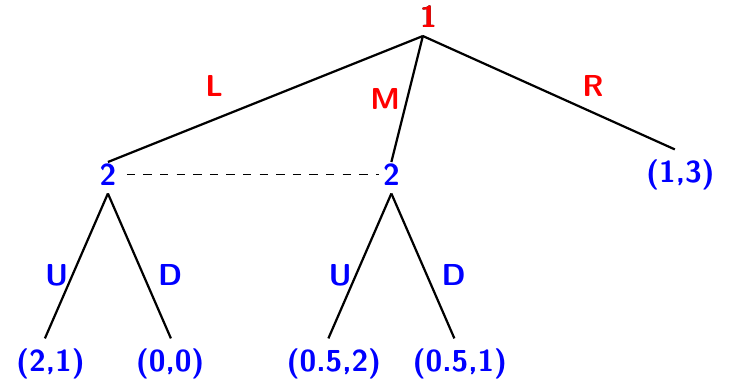
\includegraphics[
width=0.85\linewidth
]{../images/week07_01.png}

\end{center}


\begin{itemize}

\item Player 2 moves only if Player 1 chooses L or M. In that case, Player 2
\textbf{doesn't know if the choice was L or M}.

\item The two nodes connected by a dashed line form an \textbf{information set}.

\end{itemize}


\begin{definition}

\textbf{INFORMATION SET}

A set of decision nodes such that:

\begin{itemize}

\item every node in the set belongs to \textbf{one} player;

\item when the game reaches the information set, the player with the move
\textbf{cannot differentiate} between the nodes of the set.

\end{itemize}

\end{definition}


\begin{important}

Player 2 sees the same thing at both nodes, so she must choose \textbf{the same action at
both} (U at both, or D at both). A strategy chooses one action per \emph{information set}, not
per node. With perfect information (Lecture 3), every information set had one node.

\end{important}



%=========================================================
\section{Subgames with Incomplete Information}


\begin{definition}

\textbf{SUBGAME}

A subgame must include a \textbf{single initial node forming an information set} by itself,
and all its successor nodes. If a subgame includes one node of an information set, it must
include \textbf{all} the nodes of that information set.

\end{definition}


\begin{warning}

Example 1 has only \textbf{itself} as a subgame: Player 2's nodes cannot start a subgame
(their information set has two nodes). $\Rightarrow$ \textbf{SPE coincide with NE}: the SPE
refinement removes nothing.

\end{warning}



%=========================================================
\section{Example 1: Nash Equilibria}


\begin{center}
\begin{tabular}{c|cc}
$1 \backslash 2$ & U & D \\
\hline
L & \underline{(2,1)} & (0,0) \\
M & (0.5,2) & (0.5,1) \\
R & (1,3) & \underline{(1,3)} \\
\end{tabular}
\end{center}


\begin{itemize}

\item Two pure-strategy NE: \textbf{(L,U)} and \textbf{(R,D)}.

\item (R,D): against D, Player 1's best is R (1 vs 0 vs 0.5); against R, Player 2 does not
move and gets 3 whatever she plans.

\end{itemize}


\begin{warning}

\textbf{(R,D) is not credible}: once Player 2 moves (so she knows Player 1 didn't choose R),
D is \textbf{dominated}: U gives 1 instead of 0 at the L node, 2 instead of 1 at the M node.

We need a new equilibrium concept that incorporates \textbf{sequential rationality} in this
kind of game.

\end{warning}



%=========================================================
\section{Perfect Bayesian Equilibrium (PBE)}


\begin{definition}

\textbf{THE FOUR REQUIREMENTS}

\begin{enumerate}

\item \textbf{Beliefs}: at each information set with more than one node, the player who moves
has a \textbf{belief} about the probability of having reached each node ($p$ and $1-p$).

\item \textbf{Sequential rationality}: at each information set, the action taken must be
\textbf{optimal given the beliefs}.

\item On the \textbf{equilibrium path} of the game or of any of its subgames, beliefs are
determined by the \textbf{equilibrium strategies and Bayes rule}.

\item \textbf{Off} the equilibrium path in all subgames: \textbf{no restriction} on beliefs.

\end{enumerate}

\end{definition}


\begin{important}

A PBE is a SPE which in addition specifies a set of beliefs at each information set with more
than one node. \textbf{Strategies are optimal given the beliefs, and beliefs are correct given
the strategies.}

\emph{On the path} = reached with positive probability: Bayes rule gives the belief.
\emph{Off the path} = probability 0: Bayes would divide by 0, so any belief --- but the action
must still be optimal given it.

\end{important}


\begin{example}

\textbf{Example 1 solved}

\begin{itemize}

\item U gives $p \cdot 1 + (1-p)\cdot 2 = 2 - p$; D gives $p \cdot 0 + (1-p)\cdot 1 = 1 - p$.
U is better for \emph{every} $p$: Requirements 1 and 2 \textbf{kill (R,D)}.

\item Anticipating U, Player 1 plays L (2 $>$ 1 $>$ 0.5).

\item Requirement 3: Player 1 plays L, so $p = 1$.

\end{itemize}

\textbf{PBE: (L,U) with $p = 1$}.

\end{example}



%=========================================================
\section{Example 2}


\begin{center}

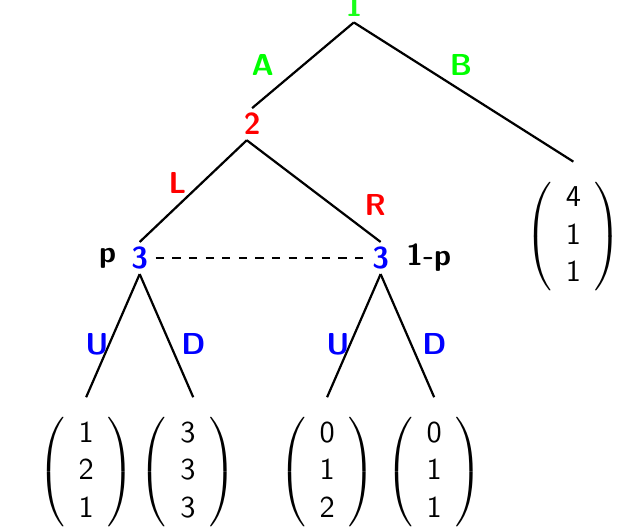
\includegraphics[
width=0.75\linewidth
]{../images/week07_02.png}

\end{center}


Payouts (Player 1, Player 2, Player 3). The game after A is a \textbf{proper subgame} (it
contains the whole information set of Player 3).


\begin{itemize}

\item In the subgame, L strictly dominates R for Player 2 (2 $>$ 1 against U, 3 $>$ 1 against
D).

\item \textbf{Requirement 3 implies $p = 1$}, consistent with Player 2's equilibrium strategy
in the smallest subgame. Then D (3) beats U (1) for Player 3.

\item The subgame gives $(3,3,3)$ $<$ 4: Player 1 plays B.

\end{itemize}


\begin{important}

\textbf{PBE is $(B, L, D)$, with $p = 1$.}

\end{important}


\begin{warning}

\textbf{Why ``or of any of its subgames''} (not on the slides): with B, Player 3's information
set is never reached in the whole game. Without Requirement 3 on subgames, $p = 0$ would be
allowed; then U is optimal and $(B, L, U)$ would pass Requirements 1--2. But Player 2 plays
L, so $p = 0$ is absurd: Requirement 3 in the subgame forces $p = 1$.

\end{warning}



%=========================================================
\section{Example 3: Beliefs with Mixed Strategies}


If Player 1's equilibrium strategy is to play L, M, R with probability
$(q_1, q_2, 1 - q_1 - q_2)$, Requirement 3 implies (Bayes rule):


\begin{formula}

\[
p = Prob(L \,|\, L \text{ or } M) = \frac{q_1}{q_1 + q_2}
\]

\end{formula}


E.g.\ (not on the slides) $(q_1, q_2) = (0.2, 0.6)$: $p = 1/4$.



%=========================================================
\section{Signaling Games}


\begin{definition}

\textbf{SIGNALING GAME}

Game of incomplete information with a \textbf{sender} and a \textbf{receiver}.

\begin{itemize}

\item The sender can be of two or more types (``strong'' or ``weak''; ``smart'' or ``dumb''),
she knows her type, the receiver cannot observe it.

\item At least one type of sender wants the receiver to know her type and sends
\textbf{signals}.

\item The receiver observes the signal, infers something about the type, and chooses
accordingly.

\end{itemize}

\end{definition}


\begin{definition}

\textbf{SEPARATING vs POOLING EQUILIBRIA}

\begin{itemize}

\item \textbf{Separating}: the ``strong'' type sends a signal strong enough that the ``weak''
type cannot match. The receiver correctly identifies the types.

\item \textbf{Pooling}: the ``weak'' type imitates the signal of the strong. Everybody sends
the same signal, the receiver learns nothing about the type.

\end{itemize}

\end{definition}


\begin{important}

A signal only says something if it is \textbf{costly}, and \textbf{more costly for the weak
type}. A free signal can be sent by anybody (``cheap talk'').

\end{important}



%=========================================================
\section{The Spence Education Game}


\begin{itemize}

\item Two players: a \textbf{job applicant} and an \textbf{employer}.

\item Nature chooses the type: ``smart'' (productivity $\theta_S$) or ``dumb''
($\theta_D$), $\theta_S > \theta_D$, 50\% each. The employer cannot observe it.

\item The applicant chooses education $e \in [0, e_{max}]$, \textbf{intrinsically useless}
but harder for the dumb: cost $e/\theta_S$ for the smart, $e/\theta_D$ for the dumb.

\item The employer observes $e$, forms a belief, and offers the salary $E[\theta|e]$
(otherwise he is out of business). Beliefs must be consistent with the applicant's strategy
on the equilibrium path.

\end{itemize}


\begin{center}

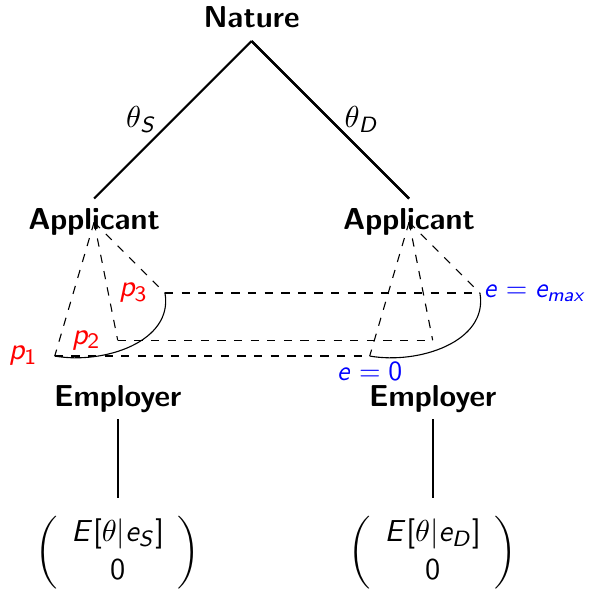
\includegraphics[
width=0.8\linewidth
]{../images/week07_03.png}

\end{center}


Each education level is an information set of the employer: seeing $e$, he does not know
which type chose it ($p_1, p_2, p_3$: his beliefs).



%=========================================================
\section{Spence: Separating Equilibrium}


The smart type chooses $e^*$ so costly for the dumb that the dumb prefers $e = 0$, even if
$e^*$ would get him the salary of a smart type:


\begin{formula}

\begin{align*}
\theta_S - \frac{e^*}{\theta_D} &< \theta_D \quad \text{(D prefers } e = 0\text{)} \\
\theta_S - \frac{e^*}{\theta_S} &> \theta_D \quad \text{(S prefers } e = e^*\text{)}
\end{align*}

\[
\Rightarrow \quad \theta_D(\theta_S - \theta_D) < e^* < \theta_S(\theta_S - \theta_D)
\]

Optimally: $e^* = \theta_D(\theta_S - \theta_D) + \epsilon$.

\end{formula}


Left side: what each type gets by \emph{imitating} the other; right side: what he gets with
his own choice. The interval is not empty because education is \textbf{cheaper for the smart}.


\begin{definition}

\textbf{BELIEFS SUPPORTING IT}

\begin{itemize}

\item On the path: $e = e^* \rightarrow p(Smart) = 1$; $e = 0 \rightarrow p(Smart) = 0$.

\item Off the path (free): $0 < e < e^* \rightarrow p(Smart) = 0$;
$e > e^* \rightarrow p(Smart) = 1$.

\end{itemize}

A worker is believed dumb if $e < e^*$, smart if $e \ge e^*$. Too costly for the dumb to
choose $e^*$ $\rightarrow$ he chooses 0; not too costly for the smart $\rightarrow$ he chooses
$e^*$.

\end{definition}


\begin{example}

\textbf{Numbers} (not on the slides): $\theta_S = 2$, $\theta_D = 1$: $1 < e^* < 2$, so
$e^* = 1 + \epsilon$.

\begin{itemize}

\item Dumb: $e = 0$ gives 1; imitating gives $2 - (1 + \epsilon) < 1$.

\item Smart: $2 - (1 + \epsilon)/2 \approx 1.5 > 1$.

\end{itemize}

\end{example}



%=========================================================
\section{Spence: Pooling Equilibria}


Unintuitive PBE in which both types choose the same $\tilde{e}$ below $e^*$. With a 50\%
prior:


\begin{formula}

\[
0 \le \tilde{e} < \frac{\theta_D(\theta_S - \theta_D)}{2}, \qquad
\text{salary} = \frac{\theta_S + \theta_D}{2}
\]

Beliefs: $e = \tilde{e} \rightarrow p = 0.5$ (the prior); $e \neq \tilde{e} \rightarrow
p(Smart) = 0$. Both types prefer $\tilde{e}$ to $e = 0$ (salary $\theta_D$):

\begin{align*}
\frac{\theta_S + \theta_D}{2} - \frac{\tilde{e}}{\theta_D} &> \theta_D \\
\frac{\theta_S + \theta_D}{2} - \frac{\tilde{e}}{\theta_S} &> \theta_D
\end{align*}

\end{formula}


\begin{warning}

The slide writes ``rather than $\theta_L$'': read $\theta_D$.

\end{warning}


\begin{definition}

\textbf{INTUITIVE CRITERION}

Even beliefs at information sets off the equilibrium path \textbf{cannot assign positive
probability to a dominated strategy}.

\end{definition}


\begin{important}

The pooling beliefs say that $e > \tilde{e}$ means ``dumb'', but no dumb type would ever take
$e > e^*$. Observing $e \ge e^*$, the employer must assign $p(Smart) = 1$; then the smart type
chooses $e^*$ and \textbf{the pooling equilibria collapse}.

\end{important}



%=========================================================
\section{Application: Online Dating}


Why do many dating sites limit the number of profiles you can like, or of invitations you can
send? \textbf{Artificial scarcity}: a limited like is a \textbf{stronger signal} of interest;
a limited invitation is costly, hence a signal of ``true interest''.


\begin{itemize}

\item Man interested (I) with probability $p$, uninterested (U) with probability $1-p$.

\item A date gives 2 to an interested man, 1 to an uninterested man.

\item The woman gets $u_I > 0$ with an interested man, $u_U < 0$ with an uninterested one.

\end{itemize}


\begin{center}

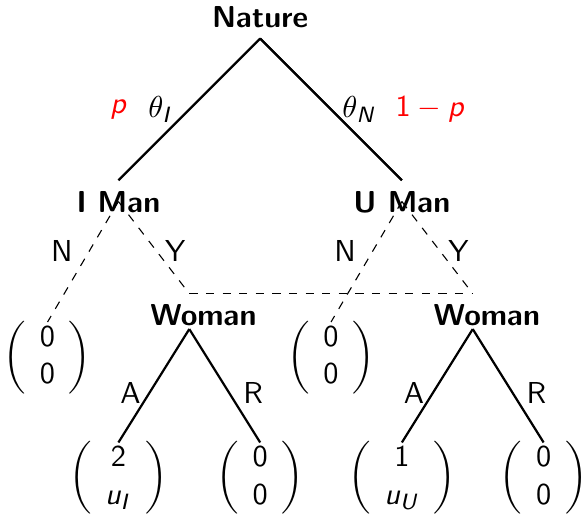
\includegraphics[
width=0.85\linewidth
]{../images/week07_04.png}

\end{center}


\begin{important}

\textbf{Without artificial scarcity} (sending is free): \textbf{pooling PBE}. All men send an
invitation; the woman's belief stays $p$; if $E[u] = p\,u_I + (1-p)\,u_U < 0$ (slides:
$p\,u_I - (1-p)\,u_U$ with $u_U$ the size of the loss), accepting is worse than rejecting
(0): \textbf{all women turn down the offer. The online dating industry does not work!}

\end{important}


\begin{center}

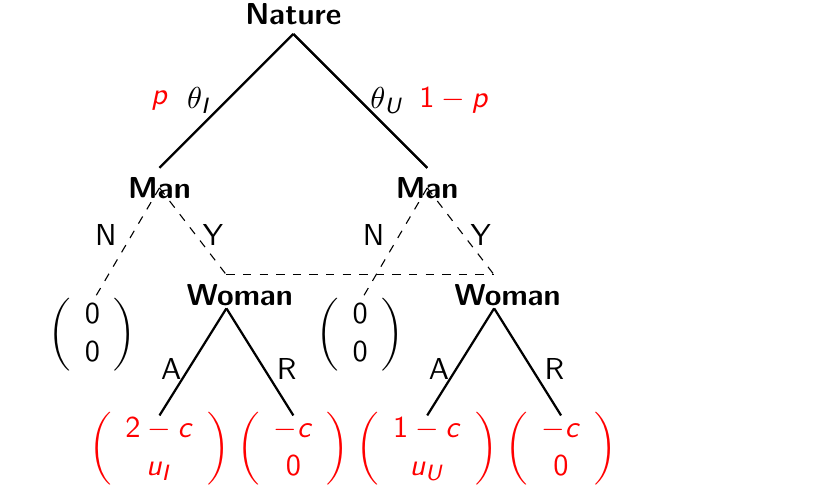
\includegraphics[
width=0.85\linewidth
]{../images/week07_05.png}

\end{center}


\begin{important}

\textbf{With artificial scarcity}, cost $c$ with $1 < c < 2$: \textbf{separating PBE}.

\begin{itemize}

\item U man: $1 - c < 0$ and $-c < 0$: he never sends.

\item I man: $2 - c > 0$ if accepted: he sends.

\item Woman: an invitation means $p = 1$, she accepts ($u_I > 0$).

\end{itemize}

\end{important}


\begin{warning}

(Not on the slides) ``Nobody sends'' is also a PBE with a pessimistic off-path belief, but
sending is dominated for type U, so the intuitive criterion forces $p = 1$ and removes it.

\end{warning}



%=========================================================
\section{Weekly Summary}


\begin{summary}

\begin{itemize}

\item \textbf{Information set}: nodes a player cannot tell apart; a subgame never cuts one,
so SPE may remove nothing.

\item \textbf{PBE}: beliefs at each information set; actions optimal given beliefs; on the
path (of the game or of a subgame) beliefs from Bayes rule; off the path free.

\item \textbf{Signaling}: separating (receiver learns the type) vs pooling (receiver learns
nothing).

\item \textbf{Spence}: $e^* = \theta_D(\theta_S - \theta_D) + \epsilon$; pooling for
$\tilde{e} < \theta_D(\theta_S - \theta_D)/2$, killed by the \textbf{intuitive criterion}.

\item \textbf{Dating}: free invitations $\rightarrow$ pooling, women refuse; costly
invitations $\rightarrow$ separating, women accept.

\end{itemize}

\end{summary}



\end{multicols}


\end{document}
